\documentclass[11pt,b5paper,twoside]{book}
\usepackage{geometry}
	\geometry{
		paper=b5paper,
		inner=16mm,         % Inner margin
		outer=24mm,         % Outer margin
		bindingoffset=10mm, % Binding offset
		top=20mm,           % Top margin
		bottom=28mm,        % Bottom margin
		%showframe,         % show how the type block is set on the page
	}
\usepackage[pdftex]{hyperref}
\usepackage{url}
\usepackage{setspace}
\usepackage{color}
\usepackage{fancyhdr}
\usepackage{tocloft}
%\usepackage{markboth}
\usepackage{fancyhdr}% http://ctan.org/pkg/fancyhdr
%\pagestyle{fancy}% Change page style to fancy
\usepackage{amsmath,blkarray}
\usepackage{ amssymb }
\usepackage{multirow}
\usepackage{lipsum}
\usepackage{tikz}
\usetikzlibrary{automata,positioning}
\usepackage{framed}
\usepackage{erewhon}
\setlength\FrameSep{0.5em}
\setlength\OuterFrameSep{\partopsep}

\singlespacing
\setlength{\parskip}{.5em}
%\renewcommand{\baselinestretch}{2.0}
\renewcommand{\contentsname}{Daftar Isi}
%\renewcommand{\partname}{Bagian}
\renewcommand{\chaptername}{Bab}
\renewcommand{\bibname}{Daftar pustaka}
%Whatever floats your boat

\renewcommand{\chaptermark}[1]{\markboth{#1}{}}
\renewcommand{\sectionmark}[1]{\markright{#1}}
\pagestyle{fancy}
\fancyhf{}
\fancyhead[LE,RO]{\thepage}
\fancyhead[LO]{\itshape\nouppercase{\rightmark}}
\fancyhead[RE]{\normalfont\nouppercase{\leftmark}}
\renewcommand{\headrulewidth}{0pt}


\newcommand{\bone}{\boldsymbol{1}}
\newcommand{\bzero}{\boldsymbol{0}}
\newcommand{\ba}{\boldsymbol{a}}
\newcommand{\bb}{\boldsymbol{b}}
\newcommand{\bd}{\boldsymbol{d}}
\newcommand{\be}{\boldsymbol{e}}
\newcommand{\bg}{\boldsymbol{g}}
\newcommand{\bh}{\boldsymbol{h}}
\newcommand{\bi}{\boldsymbol{i}}
\newcommand{\bp}{\boldsymbol{p}}
\newcommand{\bq}{\boldsymbol{q}}
\newcommand{\br}{\boldsymbol{r}}
\newcommand{\bs}{\boldsymbol{s}}
\newcommand{\bu}{\boldsymbol{u}}
\newcommand{\bv}{\boldsymbol{v}}
\newcommand{\bw}{\boldsymbol{w}}
\newcommand{\bx}{\boldsymbol{x}}
\newcommand{\by}{\boldsymbol{y}}
\newcommand{\bz}{\boldsymbol{z}}
\newcommand{\bA}{\boldsymbol{A}}
\newcommand{\bB}{\boldsymbol{B}}
\newcommand{\bC}{\boldsymbol{C}}
\newcommand{\bD}{\boldsymbol{D}}
\newcommand{\bG}{\boldsymbol{G}}
\newcommand{\bH}{\boldsymbol{H}}
\newcommand{\bI}{\boldsymbol{I}}
\newcommand{\bK}{\boldsymbol{K}}
\newcommand{\bL}{\boldsymbol{L}}
\newcommand{\bM}{\boldsymbol{M}}
\newcommand{\bN}{\boldsymbol{N}}
\newcommand{\bP}{\boldsymbol{P}}
\newcommand{\bQ}{\boldsymbol{Q}}
\newcommand{\bR}{\boldsymbol{R}}
\newcommand{\bS}{\boldsymbol{S}}
\newcommand{\bT}{\boldsymbol{T}}
\newcommand{\bU}{\boldsymbol{U}}
\newcommand{\bV}{\boldsymbol{V}}
\newcommand{\bW}{\boldsymbol{W}}
\newcommand{\bX}{\boldsymbol{X}}
\newcommand{\bY}{\boldsymbol{Y}}
\newcommand{\bZ}{\boldsymbol{Z}}
\newcommand{\cA}{{\ensuremath{\mathcal{A}}}}
\newcommand{\cI}{{\ensuremath{\mathcal{I}}}}
\newcommand{\cN}{{\ensuremath{\mathcal{N}}}}
\newcommand{\cP}{{\ensuremath{\mathcal{P}}}}
\newcommand{\cQ}{{\ensuremath{\mathcal{Q}}}}
\newcommand{\cR}{{\ensuremath{\mathcal{R}}}}
\newcommand{\cS}{{\ensuremath{\mathcal{S}}}}
\newcommand{\bpi}{\boldsymbol{\pi}}
\newcommand{\balpha}{\boldsymbol{\alpha}}
\newcommand{\bbeta}{\boldsymbol{\beta}}
\newcommand{\bDelta}{\boldsymbol{\Delta}}
\newcommand{\bepsilon}{\boldsymbol{\epsilon}}
\newcommand{\bgamma}{\boldsymbol{\gamma}}
\newcommand{\bGamma}{\boldsymbol{\Gamma}}
\newcommand{\bLambda}{\boldsymbol{\Lambda}}
\newcommand{\bmu}{\boldsymbol{\mu}}
\newcommand{\blambda}{\boldsymbol{\lambda}}
\newcommand{\bnu}{\boldsymbol{\nu}}
\newcommand{\btheta}{\boldsymbol{\theta}}
\newcommand{\Beta}{\boldsymbol{\eta}}
\newcommand{\bSigma}{\boldsymbol{\Sigma}}
\newcommand{\trace}[1]{\mbox{tr}(#1)}
\newcommand{\veco}[1]{\mbox{vec}(#1)}
\newcommand{\Rcode}[1]{{\tt #1}}
\newcommand{\R}{{\tt R}}
\newcommand{\sspace}{\textit{state space }}
\newcommand{\qed}{\hfill$\blacksquare$}

%\input{"/Users/shofiandari/Documents/Buku Ajar/prosto2018/defns.tex"}
\newtheorem{theorem}{Teorema}[section]
\newtheorem{corollary}{\textit{Corollary}}[theorem]
\newtheorem{lemma}[section]{Lemma}
\newtheorem{definition}[theorem]{Definisi}
\newtheorem{ex}[theorem]{Contoh}
\newtheorem{test}[theorem]{Latihan mandiri}



\begin{document}
\title{\LARGE{\textbf{Proses Stokastik:\\Tak Kenal Maka Tak Sayang}}}
\author{Diaz Fitra Aksioma \\ Shofi Andari}
\date{}

% General definitions for all Chapters
%-------------------------------------------------------------------------------




\frontmatter
% 1st page for the Title
%-------------------------------------------------------------------------------
\maketitle


% 2nd page, thanks message
%-------------------------------------------------------------------------------
\thispagestyle{empty}

\vspace*{\fill}
\begingroup
\begin{center}
	Untuk... \\ \textit{DFA} \\ 
	\vspace{2cm}
	Untuk Kembang Kertas \textit{crew}, yang utama dan terutama \\ \textit{SA}\\
	\vspace{2cm}
	Untuk murid-murid tercinta di Departemen Statistika ITS Surabaya \\ \textit{DFA \& SA}
\end{center}
\endgroup
\vspace*{\fill}
\newpage

% 3rd page, Kata pengantar
%-------------------------------------------------------------------------------
\chapter*{Kata pengantar}
\addcontentsline{toc}{chapter}{Kata pengantar}

\noindent "\textit{Untuk apa kita belajar mata kuliah ini?}".\par 
Pertanyaan ini sangatlah mendasar dan tidak sepatutnya diabaikan begitu saja. Kami menduga bahwa kurangnya antusiasme mahasiswa untuk belajar di kelas, apalagi di luar kelas, sebagian besar diakibatkan oleh sedikitnya pemahaman mereka akan pentingnya mata kuliah yang sedang mereka pelajari. Hal ini mendorong kami, yang juga mengalami problematika serupa ketika pertama kali belajar mengenai proses stokastik satu dekade yang lalu, untuk menyusun catatan-catatan sederhana pengantar proses stokastik. \par
Kami menyadari bahwa salah satu metode belajar terbaik yaitu dengan menyampaikan, jika terlalu berlebihan untuk disebut "mengajarkan", apa yang kita pahami kepada orang lain. Dengan menerbitkan buku ini, kami berharap dapat membantu mahasiswa statistika tingkat sarjana untuk mengenal proses stokastik secara sederhana, sekaligus membantu kami sendiri untuk menjadi guru yang lebih baik.\par
Tim penulis mengucapkan terima kasih kepada guru-guru kami, yang mengajarkan proses stokastik kepada kami pertama kali, Prof. Nur Iriawan, Haryono, M.Sc, Sri Pringit Wulandari, M.Si. dan Dr. Karin Dorman. Editor kami ...
\par
Kami berdua agar para pembaca dapat memberikan masukan, kritik, maupun saran untuk dapat memperbaiki isi buku ini. Kami juga berharap buku ini dapat bermanfaat sebaik-baiknya, baik bagi mahasiswa statistika maupun pembaca yang berminat pada pemodelan stokastik secara umum.
\\


\noindent Surabaya dan Ames, November 2018\\
\vspace{.05cm}\\
\noindent \textit{DFA} \\
\textit{SA}

% 4th page, Daftar Isi
%-------------------------------------------------------------------------------
\tableofcontents

\mainmatter

% ... page, Bab 1: Mengenal Proses Stokastik
%-------------------------------------------------------------------------------
\chapter{Mengenal Proses Stokatik}
	\section{Pengertian proses stokastik} % 1.1
	
	
	\begin{definition}[proses stokastik]
	\label{prosto}
	Sebuah proses stokastik merupakan keluarga variable random $X$, di mana $t$ merupakan parameter yang berjalan dalam himpunan indeks $\{0,1,2,..., T\}$.  
	\end{definition}

	\noindent Selanjutnya kita akan sebut variabel random $X$ sebagai $X_t$ untuk mengingatkan bahwa variabel ini merupakan fungsi terhadap $t$. Secara kolektif, random variabel ini dapat dirujuk sebagai vektor random $\bX$. Secara umum kita dapat rumuskan:
	\[ \{X_t : t \in T, X_t \in \Omega_X\}\]

	\begin{definition}[\textit{state space}]
		\label{space}
		Sebuah \sspace  $\Omega_X$ merupakan sekumpulan semua nilai dari variabel random yang bersesuaian, dalam hal ini berarti variabel random $\bX$. Dengan kata lain, \sspace  merupakan \textbf{ruang sampel} dari variabel random.  
	\end{definition}

	\noindent Sebagai contoh, jika $X_t \in [0, \infty)$ merupakan rangkaian nilai-nilai random untuk $t \in T$, maka \sspace  dari proses stokastik adalah $[0, \infty)$.

	\noindent Seringkali \textbf{\textit{index set}} $T$ ditunjukkan sebagai indeks waktu, meskipun demikian bukan berarti $T$ selalu berarti \textit{rangkaian waktu}, karena bisa jadi $T$ mewakili posisi atau perpindahan tempat. Pada kesempatan ini, mari kita sepakati bahwa semua nilai sampel yang muncul untuk $X_t$ disebut \textit{state} pada waktu $t$.

	\begin{ex}
		Suatu proses dimulai pada \textit{state} $X_1 = 3$, kemudian berubah menjadi \textit{state} $X_2 = 4$, dan pada saat $t=100$ bisa jadi menjadi $X_{100} = 500$. Bagaimana kita menuliskan notasi untuk \textit{state} bernilai $13$ saat $t = 59$?
	\end{ex}
	
	
	\section{Klasifikasi proses stokastik} %1.2
	\noindent Suatu proses stokastik dapat diklasifikan berdasarkan skala pengukuran \sspace dan \textit{index set}. Strategi pemodelannya sangat tergantung pada klasifikasi diskret/kontinu ini. Untuk proses dengan waktu (\text{index set}) bersifat diskret, $T = \{0,1,2, \dots\}$ merupakan bilangan natural. Sedangkan untuk proses dengan waktu kontinu, \text{index set} seringkali didefinisikan sebagai $T=[0,\infty)$.
	
		\begin{table}[ht] 
			\caption{Klasifikasi proses stokastik}\label{Klasifikasi proses stokastik}
			
			\centering
			\begin{tabular}{cc|cc}
%				\toprule[1.5pt]
				& & \multicolumn{2}{|c}{\textbf{State space}}  \\
				& & diskret & kontinu\\
				\hline
				\multirow{2}{*}{\textbf{Index set}} & diskret & DTMC & ...\\
				& kontinu & CTMC & proses difusi\\
				\hline
			\end{tabular}
		\\[1.5pt]
		\end{table}
	
	\section{Markov chain: apa dan mengapa} %1.3
	\noindent Sebuah \textit{proses Markov} $\{X_t\}$ adalah proses stokastik yang nilai dari $X_s$ untuk $s > t$ tidak dipengaruhi oleh nilai-nilai $X_u$, untuk $u < t$. Dengan kata lain, probabilitas dari apa pun perilaku di masa depan yang muncul dari $X_t$, ketika state saat ini diketahui, tidak dipengaruhi oleh informasi mengenai perilakunya di masa lalu. DTMC merupakan proses Markov yang memiliki \sspace berupa himpunan terbatas atau cacah, serta memiliki \textit{index set} $T \in \{0,1,2, \dots\}$. Proses ini dapat dinotasikan sebagai:

		\begin{equation}
		\begin{aligned}
		P\{X_n = i_n \mid &X_0 = i_0, X_1 =i_1, \ldots,X _{n-1}=i_{n-1}\}\\
		&= P\{X_n = i_n \mid X_{n-1}=i_{n-1}\}
		\end{aligned}
		\end{equation}
	\noindent Markov chain, dinamai demikian untuk menghormati penemunya yaitu Andrei markov, seorang ahli matematika dari Rusia yang pertama kali mempublikasikan hasil rumusannya tersebut pada tahun 1906. Di waktu yang lain, seorang matematikawan lain yang juga berkebangsaan Rusia, bernama Andrey Kolmogorov merumuskan generalisasi untuk \sspace tercacah yang tak terbatas.	Pada tahun 1953, dikembangkan suatu teknik yang disebut Markov chain Monte Carlo oleh Metropolis, Rosenbluth, Rosenbluth, Teller dan Teller dari bidang statistik fisika. 
	\section*{Latihan soal} %1.4
	\addcontentsline{toc}{section}{Latihan soal}

% ... page, Bab 2: DTMC
%-------------------------------------------------------------------------------	
\chapter{Discrete time Markov chain}

	\section{Matriks probabilitas transisi 1-step} %2.1
	%\noindent \lipsum[1-10]
	\begin{definition}(probabilitas transisi 1-step)\\
		Probabilitas transisi 1-step atau 1-langkah adalah probabilitas $X_{n+1}$ berada pada state $j$ jika diketahui $X_n$ berada pada state $i$ dan dinotasikan dengan 
		\begin{equation}
		p_{i,j}^{(n,n+1)}= P\{X_{n+1} = j \mid X_n=i\}
		\end{equation}
	\end{definition}
	di mana
	\begin{itemize}
		\item $0 \leq p_{i,j}^{(n,n+1)} \leq 1$, karena probabilitas transisi tidak lain merupakan nilai peluang (bersyarat),
		
		\item $\sum_{j=0}^{\infty}p_{i,j}^{(n,n+1)}=1$, karena rangkaian perubahan menuju semua state $j$ tidak lain merupakan aplikasi dari hukum jumlah himpunan kejadian saling lepas (exhaustive) dan saling bebas (disjoint).
	\end{itemize}

	\begin{definition} (time homogeneity)\\
		Ketika probabilitas 1-step tidak bergantung pada waktu, dengan demikian
		$$
		p_{i,j}^{(n,n+1)} =p_{i,j}
		$$
		untuk semua $n$, maka Markov chain disebut sebagai time homogenous.
	\end{definition}
	\noindent Hal ini dapat diartikan bahwa kita dapat mengabaikan kapan waktu $n$ terjadi. Di mana pun pada garis waktu \textit{index set}, probabilitas transisi dengan selisih waktu 1 satuan bernilai sama.
	
	\[
	\mathbf{P}= 
	\begin{blockarray}{l *{6}{c}}
	&0 & 1 & 2 & \dots & j & \dots \\
	\begin{block}{c[cccccc]}
	0& p_{00} & p_{01} & p_{02} & \dots & p_{0j} & \dots \\
	1& p_{10} & p_{11} & p_{12} & \dots & p_{1j} & \dots \\
	2 & p_{20} & p_{21} & p_{22} & \dots & p_{2j} & \dots \\
	\vdots & \vdots & \vdots & \vdots & \dots & \vdots &\dots \\
	i & p_{i0} & p_{i1} & p_{i2} & \dots & p_{ij} & \dots \\
	\vdots & \vdots & \vdots & \vdots & \dots & \vdots & \ddots\\
	\end{block}
	\end{blockarray}
	\]
		
	\begin{ex} (DNA sequence). \label{DNAseq} 
		Misal $X_i$ menotasikan nukleosida di posisi $i$ pada genome. \textit{Index set} $T=\{0,1,2,\dots\} $ bersifat diskret dan menunjukkan posisi. \text{State space} diskret dan terbatas untuk $\bX$ adalah $\Omega_X = \{0,1,2,3\}$, dengan $A=0, C= 1, G=2, T=3$ (meskipun seringkali definisi ini diabaikan dan notasi yang dipakai disederhanakan menjadi, misalnya, $X_i = A$).\\
		Misalkan nuklesida selanjutnya bergantung hanya pada nukleosida yang muncul tepat sebelumnya, dan bukan pada nukleosida-nukleosida sebelumnya (\textit{Makrov chain property}).\\
		Diberikan $p_{ij}$ merupakan probabilitas dari nukleosida $j \in \Omega_X$ diketahui nukelosida $i \in \Omega_X$ telah muncul sebelumnya. Maka matrix Markovnya adalah
		\[
		\mathbf{P}= 
		\begin{blockarray}{l *{4}{c}}
		&0 & 1 & 2 & 3  \\
		\begin{block}{c[cccc]}
		0& p_{AA} & p_{AC} & p_{AG} & p_{AT}  \\
		1& p_{CA} & p_{CC} & p_{CG} &p_{CT}\\
		2 & p_{GA} & p_{GC} & p_{GG} & p_{GT}  \\
		3 & p_{TA} & p_{TC} & p_{TG} & p_{TT} \\
		\end{block}
		\end{blockarray}
		\]
		di mana $p_{ii} = 1 - \sum_{j \in \Omega_X \setminus i} p_{ij}$.
	\end{ex}
	
	%\lipsum[1-10]
	
	\section{Matriks probabilitas $n$-step} %2.2
	
	\begin{definition}
		Probabilitas $p_{ij}^{(n)}$ menunjukkan proses perubahan state $i$ menuju state $j$  dalam $n$ transisi. Atau
		\begin{equation}
		p_{ij}^{(n)} = P\{ X_{n+k} = j \mid X_k = i\}
		\end{equation} 
		untuk $n \geq 0$ dan state $i,j \in \Omega_X$.
	\end{definition}
	Berdasarkan kasus 1-step, kita dapat mendefinisikan probabilitas transisi $n$-step sebagai $P^{(n)} = \big(p_{ij}^{(n)}\big)$.
	
	
		\subsubsection{Persamaan Chapman-Kolmogorov}
			
			\begin{theorem}(Chapman-Kolmogorov).
				\begin{equation}
				p_{ij}^{(n+m)}=\sum_{k=0}^{\infty}p_{ik}^{(n)}p_{kj}^{(m)}
				\end{equation}
				untuk semua $n,m \geq 0$ dan semua state $i,j$.
			\end{theorem}
		\noindent \textit{Pembuktian}:\\
			\begin{equation*}
			\begin{aligned}
				  p_{ij}^{(n+m)} &= P\{ X_{n+m} = j \mid X_0 = i\}		\text{(			karena } P\{ X_{n+m+0} = j \mid X_0 = i\}\text{)}\\
				  &= \sum_{k=0}^{\infty} P\{ X_{n+m} = j \mid X_n = k,X_0 = i\} P\{X_n = k \mid X_0 = i\}\\
				  &= \sum_{k=0}^{\infty} p_{kj}^{(m)}p_{ik}^{(n)}
			\end{aligned}
			\end{equation*}
		\qed\\
		
		
		\noindent Persamaan Chapman-Kolmogorov ini dapat disederhanakan menjadi:
		$$
		\mathbf{P}^{(n+m)} = \mathbf{P}^{(n)}\mathbf{P}^{(m)}.
		$$	
		
		\noindent Selain itu, melalui induksi matematika (\textcolor{red}{should we show this?}), kita dapat menunjukkan bahwa 
		$$
		\mathbf{P}^{(n)} = \mathbf{P}^n.
		$$
		
	\begin{ex} \label{RYseq1} (Sequence R/Y ordo pertama).
		Misalkan terdapat dua state Markov chain, yaitu R untuk purin dan Y untuk pirimidin\footnotemark, yang memiliki matriks probabilitas 1-step sebagai berikut:
		\footnotetext{Purin (atau $purine$, disimbolkan $R$) adalah kelompok nukleosida A dan C, sedangkan pirimidin (atau $pyrimidine$, disimbolkan $Y$) adalah G dan T } 
		\[
		\mathbf{P}= 
		\begin{blockarray}{l *{2}{c}}
		&R & Y \\
		\begin{block}{c[cc]}
		R& p_{RR} & p_{RY} \\
		Y& p_{YR} & p_{YY} \\
		\end{block}
		\end{blockarray} =
		\begin{blockarray}{l *{2}{c}}
		&R & Y \\
		\begin{block}{c[cc]}
		R& 0.7 & 0.3 \\
		Y& 0.4 & 0.6 \\
		\end{block}
		\end{blockarray} 
		\]
		Tentukan probabilitas bahwa ditemukan purin pada posisi ke-4 di depan, diketahui purin ada pada posisi saat ini?\\
	
		\noindent\underline{Solusi:}\\
		Kita memerlukan $\mathbf{P}^4$, tetapi cara mudah untuk mendapatkannya yaitu dengan menghitung $\mathbf{P}^2$ terlebih dahulu:
		$$
		\mathbf{P}^2 = \mathbf{P}.\mathbf{P}=
		\begin{blockarray}{l *{2}{c}}
		&R & Y \\
		\begin{block}{c[cc]}
		R& 0.61 & 0.39 \\
		Y& 0.52 & 0.48 \\
		\end{block}
		\end{blockarray} 
		$$
		sehingga
		$$
		\mathbf{P}^4 = \mathbf{P}^2.\mathbf{P}^2=
		\begin{blockarray}{l *{2}{c}}
		&R & Y \\
		\begin{block}{c[cc]}
		R& 0.5749 & 0.4251 \\
		Y& 0.5668 & 0.4332 \\
		\end{block}
		\end{blockarray}.
		$$
		Nilai probabilitas yang kita cari (probabilitas bahwa ditemukan purin pada posisi ke-4 di depan, diketahui purin ada pada posisi saat ini) adalah $p_{RR}^4 = 0.0.5749$. Hal ini dapat diinterpretasikan bahwa kira-kira terdapat 57\% peluang kita akan menemukan purin di 4 posisi selanjutnya dalam DNA sequence tersebut.
	\end{ex}

	\begin{test} (lanjutan sequence R/Y ordo pertama)
		...
	\end{test}
	
	\section{Distribusi state inisial}
	\noindent Dalam rangka menghitung probbabilitas tak bersyarat, seperti "Berapa probabilitas $R$ di posisi $j$?", kita memerlukan apa yang disebut distribusi state inisial.
	
	\begin{definition}(distribusi state inisial).
		Distribusi state inisial adalah distribusi probabilitas yang didefinisikan untuk state pertama yang terjadi atau muncul pada proses, atau dinotasikan sebagai $X_0$.
		$$
		P{X_0 = i} = \alpha_i
		$$
		untuk semua $i=0,1,2,\dots \in \Omega_X$
	\end{definition}

	\noindent Perlu diingat bahwa
	\begin{itemize}
		\item Sebuah Markov chain disebut "fully specified" apabila kita telah mengetahui matriks probabilitas transisi dan distribusi probabilitas inisialnya.
		
		\item Jika kita memiliki state sebanyak $m$ dalam Markov chain, maka banyaknya parameter yang kita miliki adalah %$m(m-1)$%
	\end{itemize}

	\noindent Mari kita kembali pada pembahasan probabilitas tak bersyarat. Ingat bahwa ada dua hal yang harus kita ketahui untuk menentukan probabilitas ini. Masih ingat apa saja dua hal tersebut?\\
	% (1) Matriks probabilitas transisi dan (2) distribusi probabilitas inisial
	Menghitung probabilitas state $j$ pada waktu tertentu $n$:
	\begin{equation} \label{tak-bersyarat}
	\begin{aligned}
	P\{X_n=j\} &= \sum_{i=0}^{\infty} P\{X_n = j \mid X_0 = i\} P\{X_0=i\}\\
	& = \sum_{i=0}^{\infty} p_{ij}^{(n)}\alpha_i
	\end{aligned}
	\end{equation}
	
	\noindent Dengan demikian, kita dapat menarik persamaan \ref{tak-bersyarat} menjadi bentuk umum:
	\begin{equation*}
	\begin{split}
	P\{X_0 = i_0, X_1 = i_1, \dots, X_n = i_n\} &\quad =\\
	 P\{X_0 = i_0\} P\{X_1 = i_1 \mid X_0 = i_0\}P\{X_2 = i_2 \mid X_1 = i_1,X_0 = i_0\} \\\dots P\{X_n = i_n \mid X_{n-1} = i_{n-1} ,X_1 = i_1,X_0 = i_0\} &\quad =\\
	 P\{X_0 = i_0\} P\{X_1 = i_1 \mid X_0 = i_0\}\dots P\{X_n = i_n \mid X_{n-1} = i_{n-1}\},
	\end{split}
	\end{equation*}
	dan dengan memasukkan parameter-parameter yang kita miliki (apa saja, masih ingat kan?), kita peroleh:
	\begin{equation}
		P\{X_0 = i_0, X_1 = i_1, \dots, X_n = i_n\} = \alpha_{i_0} p_{i_0i_1}p_{i_1i_2}\dots p_{i_{n-1}i_n}
	\end{equation}
	
	\begin{ex} (Sequence R/Y). Merujuk pada \textbf{Contoh \ref{RYseq1}}, tentukan probabilitas sebuah pirimidin pada posisi ke-empat selanjutnya, jika diketahui terdapat 90\% peluang $Y$ muncul di posisi awal?
	
	\noindent \underline{Solution:}\\
	Karena kita hanya memiliki dua state dan $\sum_{\forall i} \alpha_i=1$, maka kita dapat pastikan bahwa jika $\alpha_1=0.9$ maka $\alpha_0=1-0.9=0.1$. \\
	Dengan memanfaatkan persamaan untuk probabilitas tak bersyarat \ref{tak-bersyarat}, kita memperoleh:
		\begin{equation*}
		\begin{aligned}
		P\{X_4 = 1\} &=\sum_{i=0}^{1} p_{i1}^{(4)} \alpha_i\\
		&=p_{01}^{(4)}\alpha_0 +p_{11}^{(4)}\alpha_1\\
		&=0.4251 \times 0.1 + 0.4332 \times 0.9 \\
		&= 0.43239 
		\end{aligned}
		\end{equation*}
	\end{ex}

	\begin{test} \label{lampu1}
	Dalam suatu rangkai lampu yang akan dipasang pada perayaan 17-Agustus, dalam satu rangkaian hanya akan ada lampu berwaerna merah $R$, biru $B$, hijau $G$, dan kuning $Y$. Asumsikan warna nyala lampu merupakan state set. Diketahui dua informasi mendasar untuk mendefinisikan suatu Markov chain sebagai berikut:
	$$
	\mathbf{P}=
	\begin{blockarray}{l *{4}{c}}
	& r & b & g & y \\
	\begin{block}{c[cccc]}
	r& \dots & 0.2 & 0.2 & 0.2 \\
	b&  0.2 & \dots & 0.2 & 0.2 \\
	g&  0.2 & 0.2 & \dots & 0.2 \\
	y&  0.2& 0.2 & 0.2 &\dots \\
	\end{block}
	\end{blockarray}.
	$$
	Probabilitas inisial untuk semua state memiliki nilai yang sama.
	\begin{enumerate}
		\item Anda tentu menyadari bahwa bagian elemen diagonal matriks $\mathbf{P}$ belum lengkap. Anda dapat melengkapinya terlebih dahulu untuk menyelesaikan permasalahan-permasalahan berikutnya.
		\item Tuliskan probabilitas inisial untuk semua state $i \in \{R,B,G,Y\}$.
		\item Tentukan $P\{RR\}$.		
		\item Tentukan $P\{RRRRRR\}$.		
		\item Tentukan $P\{RNR\}$, dengan $N$ menunjukkan sembarang state.		

	\end{enumerate}
	\end{test}

	\begin{center}
		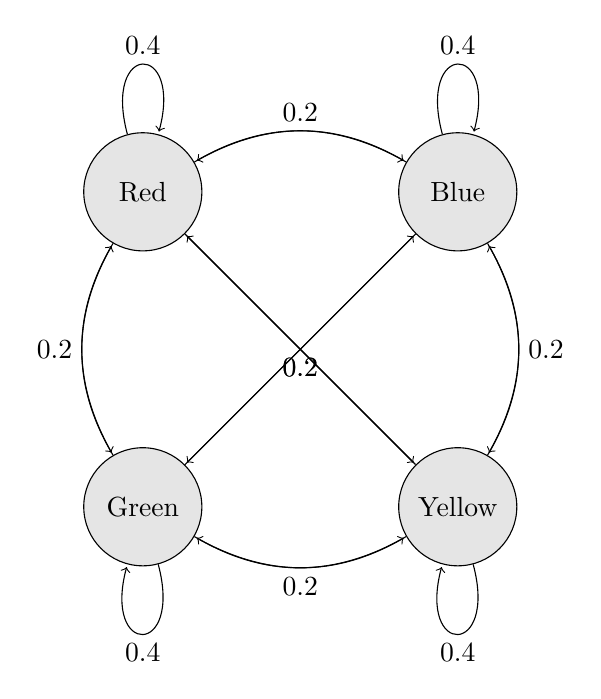
\begin{tikzpicture}
		\tikzset{node style/.style={state, 
				minimum width=1.5cm,
				%ine width=1mm,
				fill=gray!20!white}}
			
		% Draw the states
		\node[node style] at (0,0)       (r) {Red};
		\node[node style] at (4,0) (b) {Blue};
		\node[node style] at (0,-4) (g) {Green};
		\node[node style] at (4,-4) (y) {Yellow};
		
		% Connect the states with arrows
		\draw[every loop]
		(r) 	edge[bend left] node {} (b)
		 		edge[] node{} (y)
		 		edge[bend right, left] node{0.2} (g)
		 		edge[loop above] node{0.4} ()
		(b) 	edge[bend right,above] node {0.2} (r)
		 		edge[bend left,right] node {0.2} (y)
		 		edge[] node {} (g)
		 		edge[loop above] node{0.4} ()
		(g) 	edge[bend left, right] node {} (r)
				edge[below] node {0.2} (b)
				edge[bend right,below] node {0.2} (y)
				edge[loop below] node[below]{0.4} ()
		(y) 	edge[bend right] node {} (b)
				edge[below] node {0.2} (r)
				edge[bend left] node {} (g)
				edge[loop below] node[below]{0.4} ();
		
		\end{tikzpicture}
	\end{center}
	\section{Sifat-sifat DTMC} %2.3
	
		\subsubsection{Fungsi likelihood}
		
		\begin{test}\label{lampu2}
			Merujuk pada Latihan \ref{lampu1} sebelumnya, 
			\begin{itemize}
				\item Tentukan likelihood untuk warna lampu merah-merah-biru-hijau-kuning-merah-merah-merha-kuning-hijau-biru-merah-kuning-hijau-hijau-hijau-biru-kuning.
				
				\item Tentukan ... jika kedua rangkaian saling bebas
			\end{itemize} 
		\end{test}
		\subsubsection{Markov chain ordo tinggi}
		
		\subsubsection{Penggunaan Markov chain}
		
		\subsubsection{\textit{Irreducibility}}
		
		\noindent Terdapat satu bahasan yang sangat penting untuk kita ketahui saat mempelajari proses stokastik, yaitu mengenai apa yang terjadi pada suatu $rantai$ proses yang berjalan sangat $lama$, seperti genome yang sangat panjang,  kejadian hujan/tidak-hujan per hari dalam setahun, dan aplikasi lain-lain yang memanfaatkan Markov chain. Dalam sub-bab ini, kita akan mengupas mengenai apa yang terjadi, meskipun kita tidak akan mengulas lengkap pembuktian matematisnya, paling tidak untuk membantu kita memahami 'behind-the-scenes', tidak hanya menjadi pengguna rumus. \\
		
		\noindent Didefinisikan transisi 0-step sebagai Kronecker delta, atau $p_{ij}^{(n)} = \delta_{ij}$, yang menunjukkan bahwa kita hanya akan bisa menuju ke state yang sama dengan state kita berasal. (\textcolor{red}{the heck I am talking about?})
		
		\begin{definition} ($accesible$).
			State $j$ disebut \textbf{accesible} dari state $i$ apabila $p_{ij}^{(n)} > 0$ untuk $n \geq 0$.
		\end{definition}
	
		\begin{definition} ($communicate$).
			Dua state $i$ dan $j$ disebut \textbf{communicate} jika keduanya accessible terhadap satu sama lain, dan kita tuliskan $ i \leftrightarrow j$.
		\end{definition}
		 
		 \noindent Hubungan komunikasi merupakan hubungan yang ekuivalen, dengan kata lain hubungan tersebut memenuhi tiga sifat berikut:
		 
		 \begin{itemize}
		 	\item \textbf{Reflexive}: $ i \leftrightarrow j$ karena $p_{ii}^{(0)} =1$.
		 	
		 	\item \textbf{Commutative}: Jika $ i \leftrightarrow j$ , maka $ j \leftrightarrow i$.
		 	
		 	\item  \textbf{Transitive}: Jika  $ i \leftrightarrow j$ dan $ j \leftrightarrow k$, maka $ i \leftrightarrow k$.
		 \end{itemize}
		
		\begin{definition} (class property).
			Sebuah class property adalah sifat dimana apabila suatu kondisi benar untuk satu anggota kelas, maka kondisi tersebut juga benar untuk anggota yang lain di kelas yang sama.
		\end{definition}
	
	\noindent Semua definisi tersebut akan memabnatu kita untuk sampai pada property \textbf{irreducibility} dari suatu rantai Markov.
	
	\begin{definition} (irreducible).
		Sebuah rantai Markov disebut irreducible jika terdapat satu saja kelas ekuivalen dari state-state yang ada, dengan kata lain semua state $communicate$ terhadap satu sama lain.
	\end{definition}

	\begin{ex} \label{reducibelkah}:\\
		\begin{itemize}
		\item Apakah rantai Markov ini irreducible?
		$$
		\mathbf{P}=
		\begin{bmatrix}
		\frac{1}{2} & \frac{1}{2} & 0 \\
		\frac{1}{2} & \frac{1}{4} & \frac{1}{4} \\
		0 & \frac{1}{3} & \frac{2}{3} \\
		\end{bmatrix}%=
		$$
		
		\item Bagaimana dengan yang berikut?
		$$
		\mathbf{P}=
		\begin{bmatrix}
		\frac{1}{2} & \frac{1}{2} & 0 & 0\\
		\frac{1}{2} & \frac{1}{2} & 0 & 0\\
		\frac{1}{4} & \frac{1}{4} &  \frac{1}{4} & \frac{1}{4}   \\
		0 &  0 & 0 &1
		\end{bmatrix}%=
		$$
		\end{itemize}
	\end{ex}

	\begin{framed}\noindent
		Berikut merupakan tips untuk mengecek \textit{irreducibility}:
		
		\begin{definition} (regular). Sebuah matriks probabilitas transisi $\mathbf{P}$  disebut \textbf{regular}  jika terdapat n, sedemikian hingga $\mathbf{P}^n$ semua elemen matriks bernilai positif, atau $p_{ij}^{(n)} > 0$ untuk semua $i,j \geq 0$.
		\end{definition}
	
		\begin{lemma}
		Sebuah rantai Markov dengan matriks probability transisi regular bersifat \textbf{irreducible}.
		\end{lemma}
	
		\noindent Perhatikan bahwa untuk $n$ dengan $\mathbf{P}^n >0, p_{ij}^{(n)}$ untuk semua $i, j \geq 0$, karenanya semua state $i$ di dalam \sspace bersifat $communicate$ terhadap semua state $j$ lainnya.\\
		
	\noindent	\textbf{How?}\\
		Satu cara untuk mengecek \textit{irreducibility} ialah menghitung 	$\mathbf{P}^2$, $\mathbf{P}^4$, $\mathbf{P}^8$, ... untuk mengetahui apakah element semua matriks tersebut positif.
		
		\begin{ex} (mengecek irreducibility).
			Kembali pada matriks $3 \times 3$ pada Contoh \ref{reducibelkah}
			$$
			\mathbf{P}=
			\begin{bmatrix}
				\frac{1}{2} & \frac{1}{2} & 0 \\
				\frac{1}{2} & \frac{1}{4} & \frac{1}{4} \\
				0 & \frac{1}{3} & \frac{2}{3} \\
			\end{bmatrix}%=
			$$
			...
		\end{ex}
	\end{framed}
	
		\subsubsection{Recurrence dan transient}
		\noindent Anggap rantai Markov sebagai rangkaian state tak terbatas. Apakah memungkinkan rantai Markov kembali mengunjungi state-state yang sudah dikunjungi. \\
		
		\noindent Misalkan $f_i$ adalah probabilitas kita memulai suatu rantai di state $i$, proses akan memasuki state $i$ pada waktu tertentu di masa mendatang $n>0$. Besarnya $f_i$ tidak bergantung pada $n$, ingat bahwa $f_i$ merupakan probabilitas proses kembali ke state $i$. Perlu diingat juga bahwa sebuah state $i$ bisa saja $accessible$ dari state $j$, tetapi aksesibilitas tidak menjamin 'future-visit'. Pada contoh di bawah ini, sebuah rantai yang berawal dari state 0 dapat kembali dalam dua step atau lebih, tetapi rantai ini tidak menjadi untuk kembali (jika berpindah ke state 2), sehingga $f_0 =1$. 
		
		\subsubsection{Ergodisitas}
	
	
	\section{Distribusi stationer untuk DTMC} %2.4
	
	\section*{Latihan soal} %2.5
	\addcontentsline{toc}{section}{Latihan soal}
	
% ... page, Bab 3: Proses Poisson
%-------------------------------------------------------------------------------	
\chapter{Proses Poisson}	



% ... page, Bab 4: CTMC
%-------------------------------------------------------------------------------	
\chapter{Continuous time Markov chain}	

	\section{Definisi dan bentuk umum} %4.1
	
	\noindent Sebuah proses stokastik dengan waktu yang kontinu
	\[
	\big\{ X(t) \in \Omega_X : t \geq 0 \big\}
	\]
	
	adalah sekumpulan variabel random yang didefinisikan sebagai index set kontinu, dalam hal ini adalah $t \geq 0$. Dengan mengetahui bahwa varaibel random merupakan fungsi terhadap waktu, kita dapat melihat space set sebagai himpunan diskret, proses stokastik dengan waktu kontinu di mana state space $\Omega_X \in \{A, C, G, T\}$.  Dengan demikian maka proses stokastik tersebut akan memenuhi sifat Markov
	
	\[
	P[X(s+t) = j \mid X(s) = i, X(u), o \leq u < s] = p[X(s+t)=j \mid X(s) = i]
	\]
	
	dengan demikian proses stokastik disebut rantai Markov waktu kontinu, atau continuous tine Markov chain (CTMC).
	
	Perhatikan Gambar 1 berikut. Dari waktu $ 0 \leq t \leq 1$, state space $\Omega_X \in \{A, C, G, T\}$ berubah pada ...
	
	
	
	\section{Kolmogorov Backwards Equation} %4.2

	\noindent Untuk menghitung likelihood yang disample secara sporadis dari CTMC, kita memerlukan fungsi probabilitas transisi $p_{ij} (t)$. Terdapat dua langkah untuk mendapatkannya:\\
	
	Pertama, menentukan ekspresi yang paling mendekati $p_{ij} (h)$ untuk $h$ yang sangat kecil. Dengan demikian, kita dapat mengadopsi sistem persamaan diferensial biasa (ordinary differential equations) di mana $p_{ij} (t)$. Untuk beberapa kasus, sangat memungkina untuk secara analitik menyelesaikan sistem persamaan.  Sedangkan pada kesempatan yang lain, kita hanya bisa menggunakan solusi numerik. Berikut ini kita hanya akan membahas mengenai solusi numerik saja.
	
	
	\section{Distribusi stationer untuk CTMC} %4.3
	
	\noindent Fenomena bahwa $\bP (t) \rightarrow \bP$ dengan baris yang konstan seharusnya bukan hal yang mengejutkan. Kita mendapati fenomena yang sama denan DTMC.  Dengan semakin bertamabhnya $t$, state inisial pada akhirnya akan terlupakan dan CTMC akan mendekati distribusi limit (limiting distribution) yang hanya akan bergantung pada state saat ini
	
	\[
		\lim\limits_{t \rightarrow \infty} p_{ij}(t) = \pi_j.
	\]
	
	Limit ini tidak selalu ada, tetapi untuk model evolusi, keberadaan distribusi limit merupakan standar. Akan tetapi, bahkan saat distribusi limit tidak ada, distribusi stasioner bisa jadi tetap dapat ditentukan. Berikut cara memperolehnya.  (note: bahwa dist stasioner $\neq $  dist limit)
	
	\begin{theorem} (distribusi stasioner)\\
		Jika distribusi distribusi $\boldsymbol{\pi}$ untuk \hspace{0.08cm} $ \Omega_X$ sedemikian hingga $\boldsymbol{\pi}^T =\boldsymbol{\pi}^T \bP(t)$ untuk semua $t > 0$ dan $\sum_{i \in \Omega_X} \pi_i = 1$, dengan $i \in \Omega_X$, maka $\boldsymbol{\pi}$ adalah distribusi stasioner.
	\end{theorem}
	
	
	Teorema di atas tidak terlalu bermanfaat, karena kita harus memastikan bahwa  $\boldsymbol{\pi}$ memenuhi persamaan untuk semua $t >0 $, tetapi lemma berikut dapat memberikan hasil yang lebih berguna untuk tujuan yang sama: mendapatkan distribusi stasioner.
	
	\begin{lemma}
		Distribusi stasioner memenuhi $\boldsymbol{0}^T  = \boldsymbol{\pi}^T \bQ$.
	\end{lemma}	

	\noindent Bukti: ?
	Bagaimana mengetahui apakah distribusi stasioner memang ada? Dengan memeastikan bahwa elemen-elemen dari matriks $\bQ$ marupakan nilai-nilai yang positif.
	
	\section{Aplikasi penggunaan CTMC dalam pemodelan evolusi} %4.4
	\underline{Mengenal matriks $\bQ$}\\
	
	
	\noindent Kembali menilik pada KBE, matriks $\bQ$ merupakan matriks yang memenuhi $\bP^T (t) = \bQ \bP(t)$.
	Terdapat beberapa referensi untuk menenetukan matriks $\bQ$. Salah satu yang umum digunakan untuk awal mempelajari pemodelan evolusi adalah model Jukes-Cantor (JC69). Model ini mengasumsikan bahwa semua mutasi yang mungkin terjadi memiliki rate yang sama, kita sebut $\mu$. 
	
	\noindent Beberapa jenis model lain yaitu K80, Felsentein atau F84, dan GTR (general time reversible)
	\begin{itemize}
		\item Jukes-Cantor (JC69)
		
		\item 
	\end{itemize}
	
	\begin{ex} (evolusi)\\
		Model CTMC sangat umum digunakan dalam biologi untuk memodelkan evolusi. Misalkan kita ingin mengetahui apakah dua sequence memiliki hubungan Dengan menentukan bahwa satu posisi dalam sequence yang kita percaya merupakan homolog, dan misalkan nukleosida yang diobservasi adalah $Y_1 =$ A dan $Y_2=$ A. Karena dua sequence ini berhubungan, kita percaya bahwa keduanya memiliki nenek moyang yang sama beberapa waktu lalu (common-ancestor). \\
		Sekarang saatnya kita menentukan asumsi:
		\begin{itemize}
			\item [a.] Setelah common-ancestor, garis keturunan (lineage) terbagi dan berevolusi secara \textbf{independen} terhadap satu sama lain.
			
			\item [b.] Masing-masing lineage berevolusi dengan \textbf{time homogenous CTMC}($\bQ$).
			
			\item [c.] Proses evolusi telah stasioner sepanjang waktu yang ingin kita ketahui.
		\end{itemize}
		
		\noindent Sebagai hasilnya, kita dapat menggunakan LTP untuk menentukan likelihood
		\begin{equation*}
			\begin{aligned}
			L(\bQ \mid Y_1, Y_2) &= f(Y_1, Y_2)= P(Y_1 = A, Y_2 = A)  \hspace{2cm} \text{joint pmf}\\
											& = \sum_{N \in \Omega_X} \pi_N p_{NA}(t) p_{NA} (t)= \sum_{N \in \Omega_X} \pi_N p^2_{NA} (t)
			\end{aligned}
		\end{equation*}
		
		ASumsikan bahwa $\mu t$ = 0.1. (Perhatikan bahwa $\mu$ dan $t$ selalu muncul bersamaan dalam model JC69, atau dengan kata lain kedua variabel bersifat confounded.)
		
		
	\end{ex}
	
	\section*{Latihan soal} %3.5
	\addcontentsline{toc}{section}{Latihan soal}


%\bibliography{prosto}


\end{document}